\pagenumbering{arabic}

\chapter{Images and Videos}

\textbf{Definition of "Computer Vision":}\\
Is the science and technology of machines that see, where“see” in this case means that the machine is able to extract information from an image that is necessary to solve some task. The image data can take many forms, such as video sequences, views from multiple cameras, or multidimensional data from a medical scanner.

Some examples of applications of computer vision include systems for controlling processes, like an industrial robot or an autonomous vehicle, detecting events as for visual surveillance or people counting, or again organizing information for example for indexing databases of images and image sequences, even modeling objects or environments like in industrial inspection, medical image analysis or topographical modeling and interaction as the input to a device for computer-human interaction.

\begin{figure}[h]
    \centering
    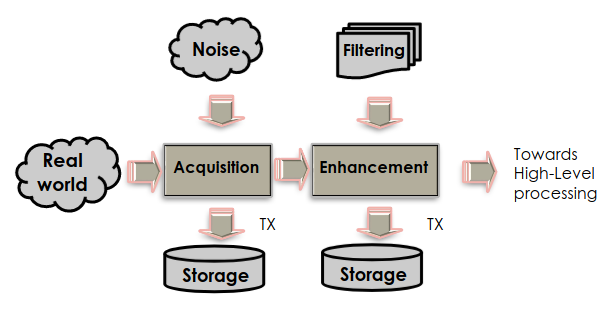
\includegraphics[scale=0.5]{Figures/ProcessingChain.png}
    \caption{The processing chain(The first part is more about signal and video, in this course we'll focus mainly on the second half)}
    \label{fig:enter-label}
\end{figure}

\textbf{Acquisition}
It refers to the process of transferring a portion of the real 3D world onto a 2D surface bringing a continuous-parameter real world into a discrete-parameter one. 
The acquisition process is the first step in the processing chain and it is the transformation of a physical signal into an electrical one, by means of a sensor. 
Where the sensor is a device that responds to a physical stimulus (light, heat, pressure, etc.) and produces an electrical signal. 
PS: The representation is in a standard format.
\\
\textbf{Digital Images}
A digital image is a representation of a two-dimensional image as a finite set of digital values, called picture elements or pixels. 
The digital image contains a fixed number of rows and columns of pixels and so is a collection of coordinates. Pixels are the smallest individual element in an image, a single pixel represent a projection of a portion of the real world, holding quantized values that represent the brightness of a given color at any specific point. Pixels can be \textbf{Grayscale} or \textbf{Color}. 
Grayscale images are represented by a single component, typically 8bit, while color images are represented by three components, typically 24bits.
\\
\textbf{Sampling}
Is the process of converting a continuous signal into a discrete signal. This is because the "real world" is a continuous function, and computers are digital. Analog video is a 1-D continuous function where one spatial dimension is mapped onto time by means of a scanning process, while digital video is instead sampled in a three dimensions (2D spatial and 1D temporal).
\\
\begin{figure}[h]
    \centering
    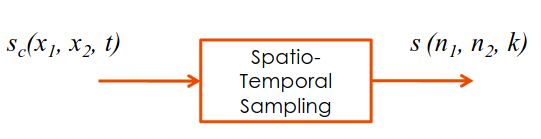
\includegraphics[scale=0.5]{Figures/Sampling.png}
    \caption{Sampling}
    \label{fig:enter-label}
\end{figure}

\textit{In a Nutshell:}
\begin{itemize}
    \item Continuous signal \[ s_c(x_1, x_2)\]
    \item Spatial rectangular sampling \[ x_1 = n_1 \bigtriangleup x_1, x_2 = n_2 \bigtriangleup x_2\]
    \item So \[ s(n_1, n_2) = s_c(n_1 \bigtriangleup x_1, n_2 \bigtriangleup x_2)\]
    \item Once we have the digital format, we can manipulate data and apply filters, change colors, store and transmit.
\end{itemize}

For what concerns handling images we need only to know that pixels are numbered starting from the top left corner (so the top left corner is the origin, arrow down for the rows and right for the columns).
The value of a pixel in a certain position is defined as \(I(r,c)\), where \(r\) is the row index and \(c\) the column one. (Start at 0 or 1, depends on you :D)
Monochrome images have values normalized in the range \([0,1]\), where 0 is black, 1 is white and the intensity is called \textit{grey level}. While color pictures have 3 channels (RGB) and the values are normalized in the same way.
\\
But what is color? It's the attribute the human visual system associates to objects, more scientifically it's a mathematical relationship that combines different wavelengths. 
It's important to check whether something we see is what we expect, to recognize objects or to distinguish similar things. For example, a white car, that for us is obviously white, for a computer is a combination of red, green and blue, moreover it has some black points for the wires, some point gray due to the street, etc.
For this reason let's talk about color perception. The human eye is like a camera with a focal length of about 20mm, where the iris controls the amount of light by adjusting the size of the pupil. 
The perception of color is possible through cones in the fovea that has around 100M receptors.  Cones have peak responses on three main wavelengths, red (700nm), green (546.1nm) and blue (435.8nm).
\\
But going back to the main topic, data can be processed locally but even transmitted remotely or archived on a storage unit. The problem is that images and videos require a lot of bandwidth, so we need to compress them with a codec.
A codec is a device or computer program for encoding or decoding a digital data stream or signal in the compressed domain. It stands for coder-decoder, and it's a way to reduce the dimension of the file (e.g JPEG, MPEG, DIVX). 
NB: Compression is lossy, so reduces quality (we lose some information) and can even introduces visual artifacts (such as blocking, blurring, chromatic aberrations(plus some noise from the sensor)). However, the loss is not a problem because the human visual system is not perfect.
NB1: Exist even lossless compression, but it's not used much.
NB2: Processing is typically done in the uncompressed domain. 
NB3: Raw images are vector of pixels.
\\
\textbf{Additive color model}
The additive color model is a method to create color by mixing the primary colors.
\begin{figure}[h]
    \centering
    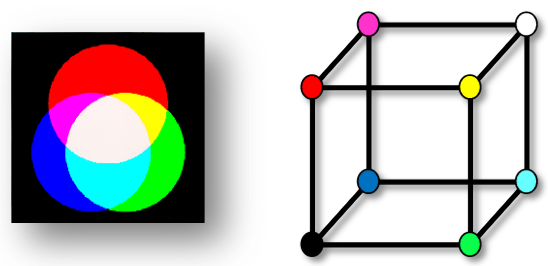
\includegraphics[scale=0.5]{Figures/AdditiveModel.png}
    \caption{Additive Color Model}
    \label{fig:enter-label}
\end{figure}

Colored beams are projected onto a black surface, then overlap so the human eye receives the stimula without generating interference, mixing the components and perceiving the resulting color.
Starting from the primary colors RGB we can obtain:
\begin{itemize}
    \item R+G = Yellow
    \item R+B = Magenta
    \item B+G = Cyan
    \item R+G+B = White
\end{itemize}
\textit{NB:Subtractive color is the inverse process.}\\
About the way colors combined, we can have:
\begin{itemize}
    \item Black: RGB(0,0,0)
    \item Green: RGB(0,1,0)
    \item Yellow: RGB(1,1,0)
    \item White: RGB(1,1,1)
    \item Gray: RGB(0.5,0.5,0.5)
\end{itemize}

Indeed, looking at the image above we can identify the gray scale along the diagonal connecting the black corner with the white corner.

NB: If we separate the three components and generate single images we notice that components are correlated, this means that the three version in grey-scale of the starting image carry almost the same amount of information.

In RGB we have a major response in the green component, while red and blue are less relevant. In addition, human eye is more sensitive to luminance and contrast variations than color so maybe a different representation would be more effective.
Indeed, more effective is the YCbCr color space, where Y, the luminance is separated from Cb and Cr that are the chrominance.
PS: YCbCr is a generalization of YUV, just a matter of conversion matrices. (TODO: Downsampling)
\\
Another color space is the HSV, where H is the hue (color), S is the saturation (brightness) and V is the value (intensity).

\begin{figure}[h]
    \begin{subfigure}{0.5\textwidth}
        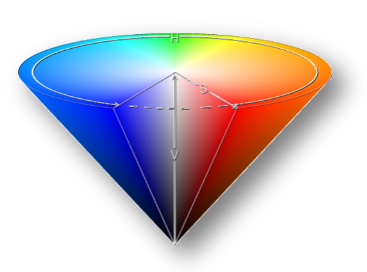
\includegraphics[scale=0.4]{Figures/HSV1.png} 
        \label{fig:subim1}
    \end{subfigure}
    \begin{subfigure}{0.5\textwidth}
        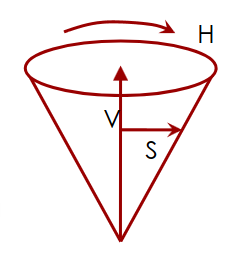
\includegraphics[scale=0.5]{Figures/HSV2.png}
        \label{fig:subim2}
    \end{subfigure}
        
        \caption{HSV Color Space}
        \label{fig:image2}
\end{figure}

Summing up just a little bit:
\begin{itemize}
    \item RGB is used in general for visualization, in displays each pixel in composed by three phosphors (CRT) or LEDs (LCD);
    \item YUV is suitable for compression since we are less sensitive to chrominance variations and U and V can be downsampled;
    \item HSV is robust for computer graphics and image analysis.
\end{itemize}
